% --------------------------------------------------------------------------- %
% --------------------------------------------------------------------------- %
\chapter{Selection Efficiencies}
\label {ch:eff}
% --------------------------------------------------------------------------- %
% --------------------------------------------------------------------------- %
Selection efficiencies is one of the ingredients needed to measure a cross
section or set an exclusion limit. The combined selection efficiency represents
the fraction of events within the acceptance that are also reconstructed and
pass the analysis selections. Acceptances here is defined as the probability
for a generated object from simulation to actually traverse through the
detector. It is customary to measure the efficiency for the various aspects of
the selections and then combine them as a measure of the total efficiency of
the analysis.

To determine where a specific model is consistent with the data, the same
analysis selections are applied to a simulated sample of this model. Here, the
simulation has been generated with a Monte Carlo generator that has been
passed through the detector simulation and then the full off-line reconstruction.
No trigger requirement is made in the simulation. Instead, we scale the
simulated events by the trigger efficiency measured for the relevant signature.
Similarly, differences exist in the efficiency of the lepton identification
and isolation requirements, as well as the b-tagging efficiency between data
and simulation. Scale factors are measured and then applied to simulation to
account for these differences.

In this chapter we describe the techniques used to measure the selection
efficiencies and acceptances. The first section describes the measurement of
the lepton efficiencies using the \tnp method and its associated uncertainties.
The next section discusses the efficiencies for the various trigger
requirements. Finally, the \dmc scale factor for b-tagged jets is shown and the
procedure used to apply it is discussed.

% --------------------------------------------------------------------------- %
% --------------------------------------------------------------------------- %
\section{Lepton Efficiencies}
\label {sec:eff_lep}
% --------------------------------------------------------------------------- %
% --------------------------------------------------------------------------- %
The efficiencies of the lepton isolation and identification requirements
(including all quality requirements) are measured with the \tnp~method
in dilepton Z events using the full 2012 dataset. The efficiency of the
identification requirements is a property of the lepton itself and is directly
applicable to the leptons in signal events. The efficiency of the isolation
requirement, however, is a strong function of all other (mainly hadronic)
activity in the event. 

In this section, the lepton efficiencies are measured and their \dmc scale
factors are computed. The systematic uncertainty for this method is assigned
for both the \tnp method itself and due to the fact that the efficiency is
measured in Z events; however, our signal events will have more hadronic
activity and are more like \ttbar events. To account for this, a short study
is also done to show the validity of measuring the efficiency in Z events and
applying them to signal-like events.

% --------------------------------------------------------------------------- %
\subsection{Tag-and-Probe Method}
\label {sec:eff_tnp}
% --------------------------------------------------------------------------- %
The basic \tnp method essentially takes advantage of the fact that we can
reconstructed \Zll events with high accuracy. We select \Zlplm events from a
lepton triggered sample by requiring opposite-sign, same-flavor leptons in
a window around the nominal Z mass, $|m_Z - \mll| < 15~\GeV$. Out of window
events are not used to extract efficiencies but are retained as sidebands to
monitor the contaminations from backgrounds. Contributions from \W and QCD
processes are found to be small. An event is ``tagged'' by requiring one lepton
to pass the full lepton selection described in Chapter~\ref{ch:evtsel} and to
be matched to an online trigger object by requiring $\DR < 0.1$ to that object.
Tagged events are classified by the other ``probe'' leptons as either
% --------------------------------------------------------------------------- %
\begin{itemize}
\item Pass: The probe passes the full selection.
\item Fail: The probe fails the full selection but passes a looser criteria
chosen to not bias the selection under study.
\end{itemize}
% --------------------------------------------------------------------------- %
The ratio of the count of the passing probe leptons to the total number of
tagged events (both passing and failing probes) is the measured efficiency. The
efficiency is extracted in bins of \pt and \aeta for both electrons and muons
separately.

% --------------------------------------------------------------------------- %
\subsubsection{Tag-and-Probe Results for Electrons}
\label {sec:eff_tnp_el}
% --------------------------------------------------------------------------- %
The electron selection efficiencies are measured in events passing the
trigger, which require one well-identified electron passing the WP80
electron ID and with $\pt>27\ \GeV$ (see Table \ref{tab:evtsel_elid}). The
tag electron is required to match the well-identified electron from the
\verb=HLT_Ele27_WP80= trigger and also to pass all the electron requirements
described in Section~\ref{sec:evtsel_el}. Additionally, the tag electron is
chosen to have a $\pt>32\ \GeV$ to eliminate turn-on effects from the trigger
efficiency. The probe electron is required to pass a simple loose selection as
follows

\begin{itemize}
\item reconstructed electron
\item $\pt > 10\ \GeV$,
\item $\aeta < 2.4$, 
\item excluding electrons with a supercluster between $1.4442 < |\eta_{SC}| < 1.566$.
\end{itemize}

The isolation efficiency is measured with the probes passing all electron
selections described in Section~\ref{sec:evtsel_el}, except for the isolation
itself. The identification efficiency is measured with probes passing the
isolation requirement. The overall efficiency is measured with probes passing
only the nominal requirements above. Results of the measurement are summarized
in Table~\ref{tab:eff_tnp_el}. The contribution from the Z events in data is
based on fitting the mass range 60-120 \GeVcc~using a simultaneous fit of
various models for the signal and backgrounds. The models used are summarized
in the following Table~\ref{tab:eff_tnp_models}. Since the kinematics of the
background shape varies in the different $\pt-\aeta$ bins, different background
shapes were chosen on a bin-by-bin basis in order to get the best fits. The
results of the \tnp show a strong dependence on the lepton \pt and a weaker but
non-negligible dependence on \aeta.
% --------------------------------------------------------------------------- %
\begin{table}[!htb]
\caption[Models used for measuring the signal or the background contribution in the \tnp~method]
{\label{tab:eff_tnp_models}
Models used for measuring the signal or the background contribution in the \tnp~method.
}
\begin{center}
\begin{tabular}{l|l}
\hline\hline
Model                                              & Usage      \\ \hline
Breit-Wigner function $\ast$ Crystal-Ball function & Signal     \\
MC-based template function                         & Signal     \\ \hline
Exponential                                        & Background \\
Exponential $\ast$ error function                  & Background \\
Polynomial                                         & Background \\
Polynomial $\times$ exponential function           & Background \\
Chebyshev Polynomial                               & Background \\
\hline\hline
\end{tabular}
\end{center}
\end{table}
% --------------------------------------------------------------------------- %
\begin{table}[!hbt]
\begin{center}
\caption[Electron efficiencies measured using the \tnp~method]
{\label{tab:eff_tnp_el}
Electron efficiencies measured using the \tnp~method.  The uncertainties are statistical only.
}
\end{center}
\resizebox{0.65\textwidth}{!}{\begin{minipage}{\textwidth}
\begin{tabular}{c|c|c|c|c|c|c|c}
\hline\hline
\backslashbox{\aeta}{\pt}     &         & $10-15$ \GeV      & $15-20$ \GeV      & $20-30$ \GeV      & $30-40$ \GeV      & $40-50$ \GeV      & $50-200$ \GeV     \\ \hline \hline
\multirow{3}{*}{$0.0-0.8$}    & MC      & 0.363 $\pm$ 0.004 & 0.503 $\pm$ 0.002 & 0.646 $\pm$ 0.001 & 0.764 $\pm$ 0.000 & 0.819 $\pm$ 0.000 & 0.841 $\pm$ 0.001 \\
                              & Data    & 0.303 $\pm$ 0.003 & 0.462 $\pm$ 0.002 & 0.617 $\pm$ 0.001 & 0.733 $\pm$ 0.000 & 0.796 $\pm$ 0.000 & 0.815 $\pm$ 0.001 \\
                              & Data/MC & 0.834 $\pm$ 0.012 & 0.918 $\pm$ 0.006 & 0.954 $\pm$ 0.002 & 0.960 $\pm$ 0.001 & 0.972 $\pm$ 0.001 & 0.969 $\pm$ 0.001 \\ \hline
\multirow{3}{*}{$0.8-1.4442$} & MC      & 0.379 $\pm$ 0.004 & 0.480 $\pm$ 0.003 & 0.600 $\pm$ 0.001 & 0.736 $\pm$ 0.001 & 0.809 $\pm$ 0.000 & 0.830 $\pm$ 0.001 \\
                              & Data    & 0.369 $\pm$ 0.008 & 0.435 $\pm$ 0.003 & 0.554 $\pm$ 0.001 & 0.688 $\pm$ 0.001 & 0.772 $\pm$ 0.000 & 0.794 $\pm$ 0.001 \\
                              & Data/MC & 0.973 $\pm$ 0.023 & 0.906 $\pm$ 0.009 & 0.923 $\pm$ 0.003 & 0.935 $\pm$ 0.001 & 0.955 $\pm$ 0.001 & 0.956 $\pm$ 0.001 \\ \hline
\multirow{3}{*}{$1.566-2.0$}  & MC      & 0.206 $\pm$ 0.004 & 0.344 $\pm$ 0.003 & 0.482 $\pm$ 0.002 & 0.615 $\pm$ 0.001 & 0.681 $\pm$ 0.001 & 0.697 $\pm$ 0.001 \\
                              & Data    & 0.197 $\pm$ 0.004 & 0.313 $\pm$ 0.003 & 0.444 $\pm$ 0.002 & 0.569 $\pm$ 0.001 & 0.647 $\pm$ 0.001 & 0.693 $\pm$ 0.001 \\
                              & Data/MC & 0.954 $\pm$ 0.028 & 0.909 $\pm$ 0.012 & 0.921 $\pm$ 0.005 & 0.924 $\pm$ 0.002 & 0.950 $\pm$ 0.001 & 0.995 $\pm$ 0.002 \\ \hline
\multirow{3}{*}{$2.0-2.4$}    & MC      & 0.199 $\pm$ 0.004 & 0.321 $\pm$ 0.004 & 0.419 $\pm$ 0.002 & 0.515 $\pm$ 0.001 & 0.576 $\pm$ 0.001 & 0.593 $\pm$ 0.002 \\
                              & Data    & 0.223 $\pm$ 0.005 & 0.303 $\pm$ 0.004 & 0.416 $\pm$ 0.000 & 0.494 $\pm$ 0.001 & 0.558 $\pm$ 0.001 & 0.575 $\pm$ 0.002 \\
                              & Data/MC & 1.119 $\pm$ 0.036 & 0.944 $\pm$ 0.015 & 0.993 $\pm$ 0.004 & 0.959 $\pm$ 0.003 & 0.968 $\pm$ 0.002 & 0.969 $\pm$ 0.004 \\ \hline \hline
\end{tabular}
\end{minipage}
}
\end{table}
% --------------------------------------------------------------------------- %

The following sources of systematic uncertainty are attributed to this
measurement: variation in the models used to fit the signal and background
distributions and measuring the isolation (Iso) and identification (ID)
components simultaneously (ID+Iso) as opposed to a factorized measurement
(ID*Iso). Varying the models for signal and backgrounds seems to make the
most significant difference to the data-to-MC scale factors in the lowest \pt
bins where the backgrounds are the largest and least understood. The effect
was sub-dominant to the difference in factorization scheme (using ID+Iso vs
ID*Iso). To show the difference between the data-to-MC scale factors using
different factorization schemes, the relative difference of the data-to-MC
scale factors when measured using ID+Iso versus ID*Iso is shown in the
following Table~\ref{tab:eff_tnp_el_fac}. As you move to lower \pt~and higher
\aeta, we see relatively larger differences between the two factorization
schemes with some differences as high as~$\sim 25\%$. The two methods offer a
trade off with the ID+Iso method accounting for the correlation between the
ID and isolation; whereas, the ID*Iso does not account for the correlation
but has a smaller background. This leads to differences in the efficiencies
between the two methods. At higher \pt~and lower \aeta, we see this effect is
mitigated with relative differences on the order of a few percent. To account
for these differences, we apply at 10\% systematic uncertainty for electrons
with $\pt<15\ \GeV$ where we saw larger differences and 5\% above where the
differences settle out.
% --------------------------------------------------------------------------- %
\begin{table}[!hbt]
\begin{center}
\caption[Electron efficiency data-to-mc scale factors measured using the \tnp~method]
{\label{tab:eff_tnp_el_fac}
Electron efficiency data-to-MC scale factors measured using the \tnp~method in
different factorization schemes. ``rel diff'' refers to the relative difference
between the two factorization schemes. The uncertainties are statistical only.
}
\end{center}
\resizebox{0.65\textwidth}{!}{\begin{minipage}{\textwidth}
\begin{tabular}{c|c|c|c|c|c|c|c}
\hline\hline
\backslashbox{\aeta}{\pt}     &          & $10-15$ \GeV      & $15-20$ \GeV       & $20-30$ \GeV       & $30-40$ \GeV       & $40-50$ \GeV       & $50-200$ \GeV      \\ \hline \hline
\multirow{3}{*}{$0.0-0.8$}    & ID*Iso   & 0.787 $\pm$ 0.022 & 0.943 $\pm$ 0.010  & 0.963 $\pm$ 0.002  & 0.969 $\pm$ 0.001  & 0.975 $\pm$ 0.000  & 0.973 $\pm$ 0.001  \\
                              & ID+Iso   & 0.834 $\pm$ 0.012 & 0.918 $\pm$ 0.006  & 0.954 $\pm$ 0.002  & 0.960 $\pm$ 0.001  & 0.972 $\pm$ 0.001  & 0.969 $\pm$ 0.001  \\
                              & rel diff & 0.055 $\pm$ 0.030 & -0.028 $\pm$ 0.013 & -0.009 $\pm$ 0.003 & -0.010 $\pm$ 0.001 & -0.004 $\pm$ 0.001 & -0.004 $\pm$ 0.002 \\ \hline
\multirow{3}{*}{$0.8-1.4442$} & ID*Iso   & 0.861 $\pm$ 0.015 & 0.910 $\pm$ 0.011  & 0.921 $\pm$ 0.002  & 0.943 $\pm$ 0.001  & 0.956 $\pm$ 0.001  & 0.950 $\pm$ 0.002  \\
                              & ID+Iso   & 0.973 $\pm$ 0.023 & 0.906 $\pm$ 0.009  & 0.923 $\pm$ 0.003  & 0.935 $\pm$ 0.001  & 0.955 $\pm$ 0.001  & 0.956 $\pm$ 0.001  \\
                              & rel diff & 0.115 $\pm$ 0.029 & -0.005 $\pm$ 0.015 & 0.003 $\pm$ 0.004  & -0.009 $\pm$ 0.001 & -0.001 $\pm$ 0.001 & 0.006 $\pm$ 0.003  \\ \hline
\multirow{3}{*}{$1.566-2.0$}  & ID*Iso   & 0.798 $\pm$ 0.028 & 0.886 $\pm$ 0.026  & 0.910 $\pm$ 0.005  & 0.928 $\pm$ 0.002  & 0.948 $\pm$ 0.001  & 0.964 $\pm$ 0.002  \\
                              & ID+Iso   & 0.954 $\pm$ 0.028 & 0.909 $\pm$ 0.012  & 0.921 $\pm$ 0.005  & 0.924 $\pm$ 0.002  & 0.950 $\pm$ 0.001  & 0.995 $\pm$ 0.002  \\
                              & rel diff & 0.164 $\pm$ 0.042 & 0.025 $\pm$ 0.031  & 0.012 $\pm$ 0.008  & -0.004 $\pm$ 0.003 & 0.002 $\pm$ 0.002  & 0.031 $\pm$ 0.003  \\ \hline
\multirow{3}{*}{$2.0-2.4$}    & ID*Iso   & 0.866 $\pm$ 0.027 & 0.929 $\pm$ 0.015  & 0.935 $\pm$ 0.005  & 0.954 $\pm$ 0.002  & 0.962 $\pm$ 0.002  & 0.955 $\pm$ 0.004  \\
                              & ID+Iso   & 1.119 $\pm$ 0.036 & 0.944 $\pm$ 0.015  & 0.993 $\pm$ 0.004  & 0.959 $\pm$ 0.003  & 0.968 $\pm$ 0.002  & 0.969 $\pm$ 0.004  \\
                              & rel diff & 0.226 $\pm$ 0.041 & 0.016 $\pm$ 0.023  & 0.058 $\pm$ 0.007  & 0.006 $\pm$ 0.004  & 0.006 $\pm$ 0.003  & 0.015 $\pm$ 0.006  \\ \hline \hline
\end{tabular}
\end{minipage}
}
\end{table}

% --------------------------------------------------------------------------- %
\subsubsection{Tag-and-Probe Results for Muons}
\label {sec:eff_tnp_mu}
% --------------------------------------------------------------------------- %
For muons, the technique for electrons is essentially repeated with appropriate
modifications for muon specific selections. The muon selection efficiencies are
measured using events that pass the \verb=HLT_IsoMu24_eta2p1= trigger which
require one isolated muon with a $\pt>24\ \GeV$. In the \tnp~analysis, the
tag muon is required to match the well-identified muon from the trigger and
also to pass all the muon requirements described in Section~\ref{sec:evtsel_mu}.
Additionally, the tag muon is chosen to have a $\pt>30\ \GeV$ to eliminate
turn-on effects from the trigger efficiency. The probe muon is required to have
% --------------------------------------------------------------------------- %
\begin{itemize}
  \item $\pt > 10\ \GeV$
  \item $\aeta < 2.4$
  \item have both the global and the particle-flow muon types.
\end{itemize}
% --------------------------------------------------------------------------- %
The isolation efficiency is measured with the probes passing all muon
selections described in Section~\ref{sec:evtsel_mu}, except for the isolation
itself. The identification efficiency is measured with probes passing the
isolation requirement. The overall efficiency is measured with probes passing
only the nominal requirements above. Results of the measurement are summarized
in Table~\ref{tab:eff_tnp_mu}. The contribution from the Z events in data
is based on fitting the mass range of 60-120 \GeVcc~using a simultaneous
fit of various models for the signal and backgrounds. The models used are
the same as those used by the electrons and are summarized in the same
Table~\ref{tab:eff_tnp_models}. Since the kinematics of the background shape
varied in the different $\pt-\aeta$ bins, different models were chosen on a
bin-by-bin basis in order to get the best fits.
% --------------------------------------------------------------------------- %
\begin{table}[hb]
\begin{center}
\caption[Muon efficiencies measured using the \tnp~method]
{\label{tab:eff_tnp_mu}
Muon efficiencies measured using the \tnp~method. The uncertainties are
statistical only.
}
\end{center}
\resizebox{0.65\textwidth}{!}{\begin{minipage}{\textwidth}
\begin{tabular}{c|c|c|c|c|c|c|c}
\hline\hline
\backslashbox{\aeta}{\pt}  &         & $10-15$ \GeV      & $15-20$ \GeV      & $20-30$ \GeV      & $30-40$ \GeV      & $40-50$ \GeV      & $50-200$ \GeV     \\ \hline\hline
\multirow{3}{*}{$0.0-1.2$} & MC      & 0.582 $\pm$ 0.003 & 0.644 $\pm$ 0.002 & 0.754 $\pm$ 0.001 & 0.857 $\pm$ 0.000 & 0.901 $\pm$ 0.000 & 0.900 $\pm$ 0.000 \\
                           & Data    & 0.556 $\pm$ 0.005 & 0.617 $\pm$ 0.002 & 0.727 $\pm$ 0.001 & 0.832 $\pm$ 0.000 & 0.881 $\pm$ 0.000 & 0.877 $\pm$ 0.001 \\
                           & Data/MC & 0.956 $\pm$ 0.010 & 0.957 $\pm$ 0.004 & 0.964 $\pm$ 0.001 & 0.971 $\pm$ 0.000 & 0.978 $\pm$ 0.000 & 0.974 $\pm$ 0.001 \\ \hline
\multirow{3}{*}{$1.2-2.4$} & MC      & 0.646 $\pm$ 0.003 & 0.682 $\pm$ 0.002 & 0.763 $\pm$ 0.001 & 0.861 $\pm$ 0.000 & 0.907 $\pm$ 0.000 & 0.895 $\pm$ 0.001 \\
                           & Data    & 0.620 $\pm$ 0.010 & 0.662 $\pm$ 0.003 & 0.731 $\pm$ 0.001 & 0.843 $\pm$ 0.000 & 0.892 $\pm$ 0.000 & 0.875 $\pm$ 0.001 \\
                           & Data/MC & 0.960 $\pm$ 0.016 & 0.971 $\pm$ 0.005 & 0.959 $\pm$ 0.001 & 0.978 $\pm$ 0.001 & 0.984 $\pm$ 0.000 & 0.977 $\pm$ 0.001 \\ \hline\hline
\end{tabular}
\end{minipage}
}
\end{table}

% --------------------------------------------------------------------------- %
Since the technique for the muons is the same as the electrons, we consider
the same sources of systematic uncertainties. As with the electrons, varying
the fitting models showed the most difference in the lower \pt~bins for the
same reason. Also, the factorization scheme was varied with the results shown
in Table~\ref{tab:eff_tnp_mu_fac}. As you move to lower \pt~and higher \aeta,
we see differences between the two factorization schemes of~$\sim
5\%$. At higher \pt~and lower \aeta, we see this effect is much smaller being
a few percent or less. To account for these differences, we apply at 5\%
systematic uncertainty for muons with $\pt<15\ \GeV$ where we saw larger
differences and 3\% above where the differences settle out.

\begin{table}[hb]
\begin{center}
\caption[Muon efficiency data-to-mc scale factors measured using the \tnp~method]
{\label{tab:eff_tnp_mu_fac}
Muon efficiency data-to-MC scale factors measured using the \tnp~method in
different factorization schemes. ``rel diff'' refers to the relative difference
between the two factorization schemes. The uncertainties are statistical only.
}
\end{center}
\resizebox{0.65\textwidth}{!}{\begin{minipage}{\textwidth}
\begin{tabular}{c|c|c|c|c|c|c|c}
\hline\hline
\backslashbox{\aeta}{\pt}  &          & $10-15$ \GeV       & $15-20$ \GeV       & $20-30$ \GeV       & $30-40$ \GeV       & $40-50$ \GeV       & $50-200$ \GeV      \\ \hline\hline
\multirow{3}{*}{$0.0-1.2$} & ID*Iso   & 0.918 $\pm$ 0.017  & 0.955 $\pm$ 0.008  & 0.965 $\pm$ 0.001  & 0.972 $\pm$ 0.000  & 0.979 $\pm$ 0.000  & 0.974 $\pm$ 0.001  \\
                           & ID+Iso   & 0.956 $\pm$ 0.010  & 0.957 $\pm$ 0.004  & 0.964 $\pm$ 0.001  & 0.971 $\pm$ 0.000  & 0.978 $\pm$ 0.000  & 0.974 $\pm$ 0.001  \\
                           & rel diff & 0.040 $\pm$ 0.021  & 0.003 $\pm$ 0.009  & -0.001 $\pm$ 0.002 & -0.001 $\pm$ 0.001 & -0.001 $\pm$ 0.000 & -0.000 $\pm$ 0.001 \\ \hline
\multirow{3}{*}{$1.2-2.5$} & ID*Iso   & 0.962 $\pm$ 0.011  & 1.034 $\pm$ 0.006  & 0.972 $\pm$ 0.001  & 0.980 $\pm$ 0.001  & 0.985 $\pm$ 0.000  & 0.980 $\pm$ 0.001  \\
                           & ID+Iso   & 0.960 $\pm$ 0.016  & 0.971 $\pm$ 0.005  & 0.959 $\pm$ 0.001  & 0.978 $\pm$ 0.001  & 0.984 $\pm$ 0.000  & 0.977 $\pm$ 0.001  \\
                           & rel diff & -0.003 $\pm$ 0.020 & -0.065 $\pm$ 0.008 & -0.013 $\pm$ 0.002 & -0.002 $\pm$ 0.001 & -0.001 $\pm$ 0.001 & -0.003 $\pm$ 0.001 \\ \hline\hline
\end{tabular}
\end{minipage}
}
\end{table}

% --------------------------------------------------------------------------- %
\subsection{Lepton Composition}
\label {sec:eff_comp}
% --------------------------------------------------------------------------- %
In the previous sub-sections, we saw there there is an uncertainty associated
with the \dmc scale factors on the lepton efficiency. Another source of
uncertainty in the efficiencies measured above stems from the fact that the
efficiency is extracted from Drell-Yan (DY) events; however, the individual
efficiencies for ID and isolation for non-DY events may differ. A Monte
Carlo study was done to measure the ID and isolation efficiencies in \Zll
with respect to $\ttbar \rightarrow \ell\nu q \ell\nu q$ events. The exact
datasets used are listed in Appendix~\ref{sec:mc_details_sm}. The denominator
selection for these efficiencies was any generator-level e/$\mu$/$\tau$ ($\tau
\rightarrow e/\mu$) which is truth matched to a W/Z boson decay at the parton
level (Pythia6 status 3) within the acceptance and $\pt > 10\ \GeV$. The
numerator selection requires that this generated level lepton is truth matched
to a reconstructed lepton of the appropriate flavor which passes the full
analysis selection outlined in Chapter~\ref{ch:evtsel}. The results from this
study are shown in Figures~\ref{fig:eff_comp_el}, \ref{fig:eff_comp_mu} and in
Tables~\ref{tab:eff_comp_el}, \ref{tab:eff_comp_mu} for electrons and muons,
respectively.
% --------------------------------------------------------------------------- %
\begin{table}[!hbt]
\begin{center}
\caption[The electron efficiency relative differences between DY and \ttbar]
{\label{tab:eff_comp_el}
The electron efficiency relative differences between DY and \ttbar~
($(\epsilon_{DY} - \epsilon_{\ttbar})/\epsilon_{DY}$). The uncertainties are
statistical only.
}
\begin{tabular}{c|c|c}
\hline\hline
\backslashbox{\pt}{\aeta} & 0.00 - 1.44       & 1.57 - 2.50        \\\hline
10 - 20 \GeV              & 0.080 $\pm$ 0.021 &  0.094 $\pm$ 0.051 \\
20 - 30 \GeV              & 0.056 $\pm$ 0.011 &  0.021 $\pm$ 0.033 \\
30 - 40 \GeV              & 0.068 $\pm$ 0.009 &  -0.013 $\pm$ 0.030\\
40 - 50 \GeV              & 0.025 $\pm$ 0.009 &  -0.003 $\pm$ 0.030\\
50 - 70 \GeV              & 0.034 $\pm$ 0.007 &  0.038 $\pm$ 0.025 \\
70 - 100 \GeV             & 0.012 $\pm$ 0.010 &  0.033 $\pm$ 0.032 \\
100- 200 \GeV             & 0.021 $\pm$ 0.014 &  -0.027 $\pm$ 0.049\\ 
\hline\hline
\end{tabular}
\end{center}
\end{table}
% --------------------------------------------------------------------------- %
\begin{figure}[!hbt]
\begin{center}
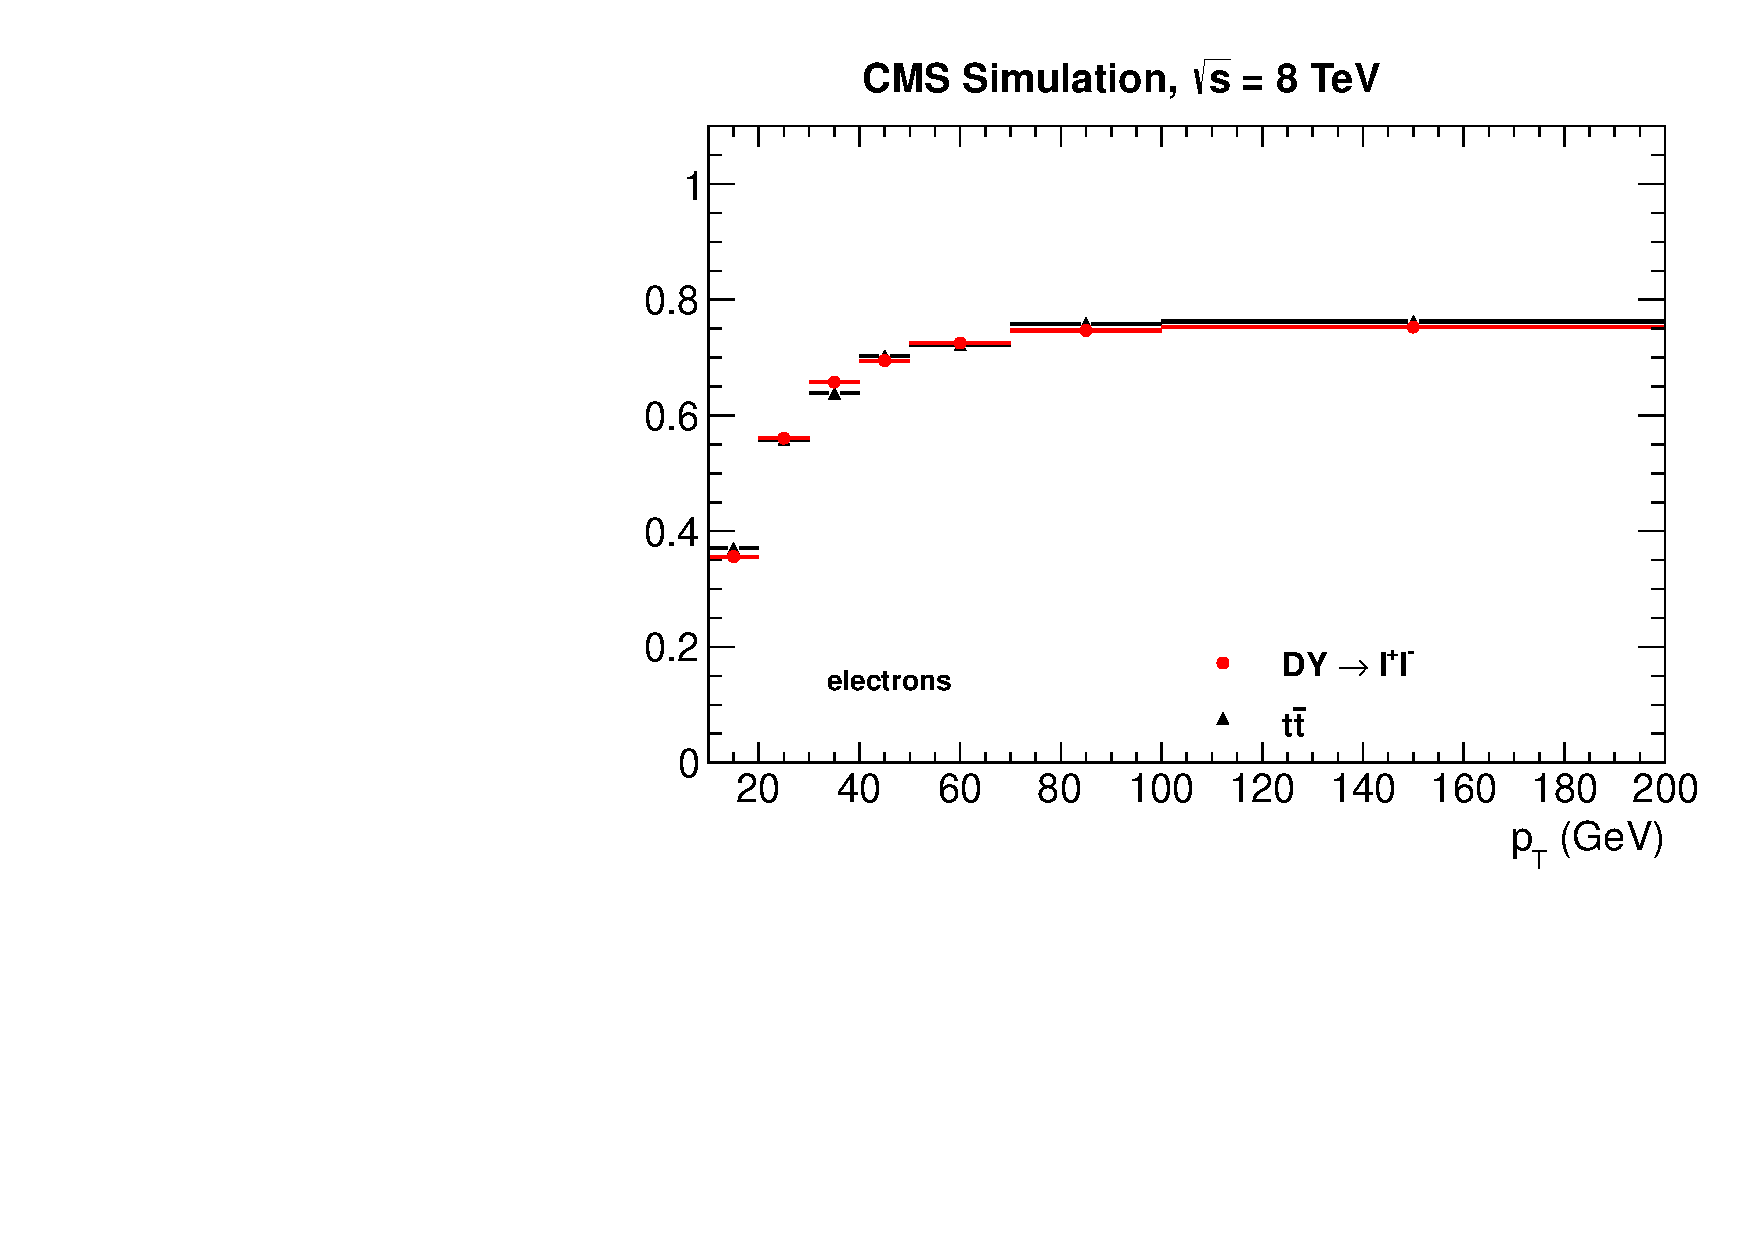
\includegraphics[width=0.49\linewidth]{p_eff_el_vs_pt}
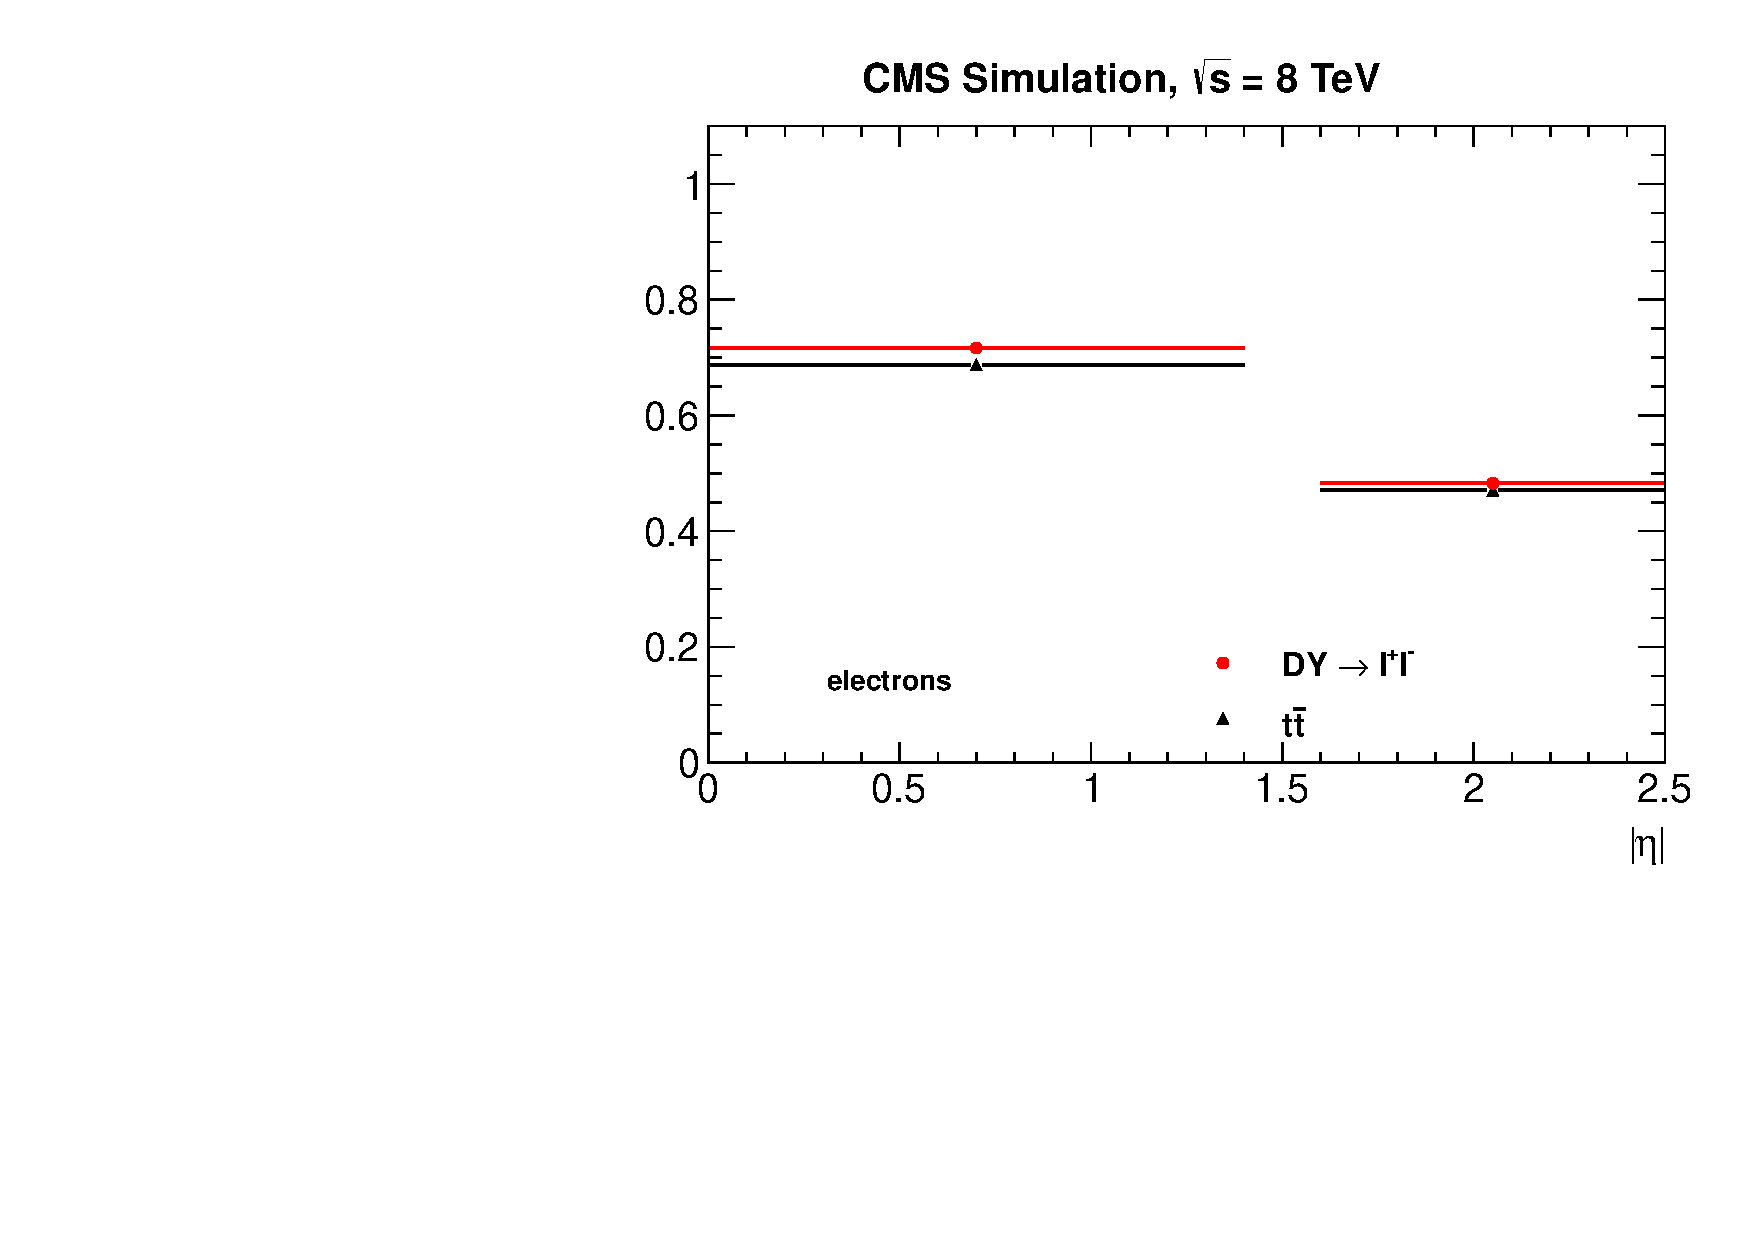
\includegraphics[width=0.49\linewidth]{p_eff_el_vs_eta}
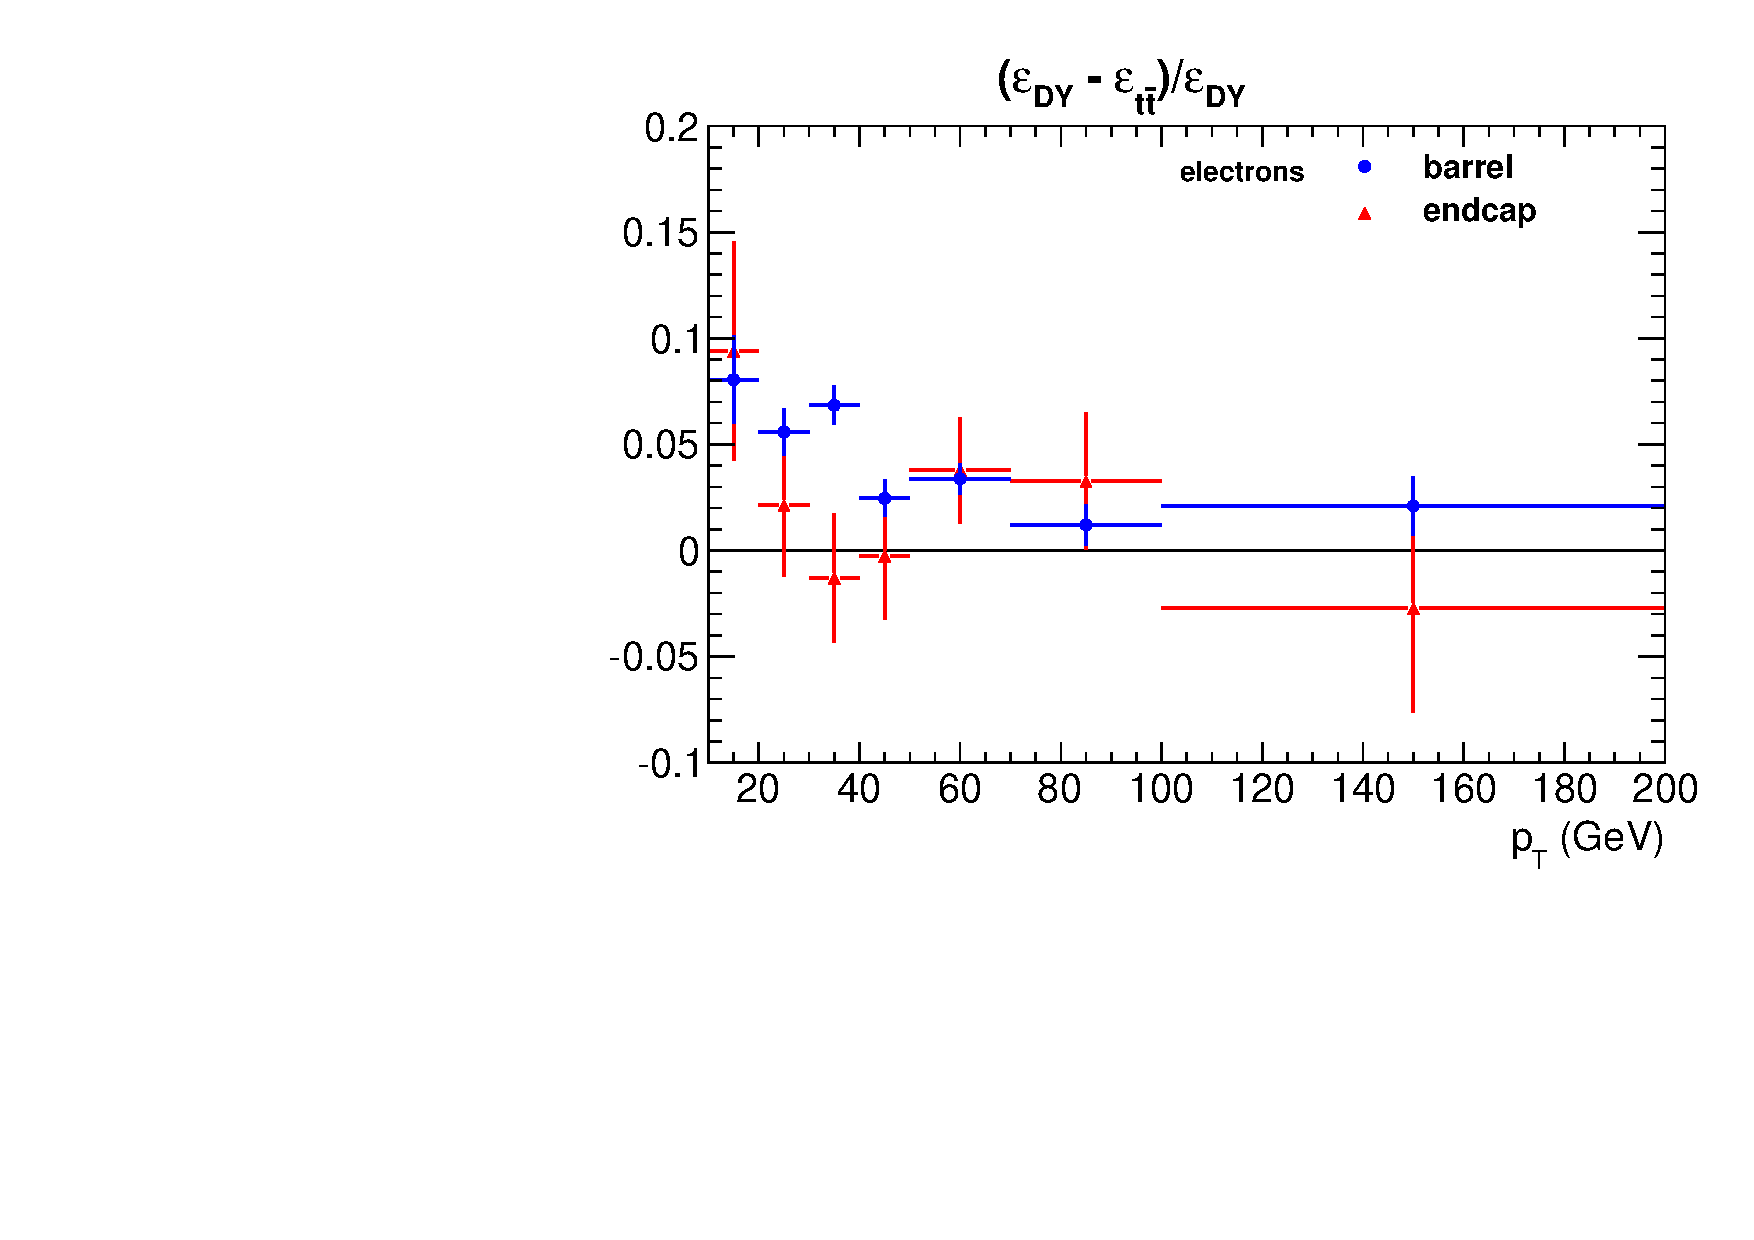
\includegraphics[width=0.49\linewidth]{p_eff_el_rel_diff_vs_pt_compare}
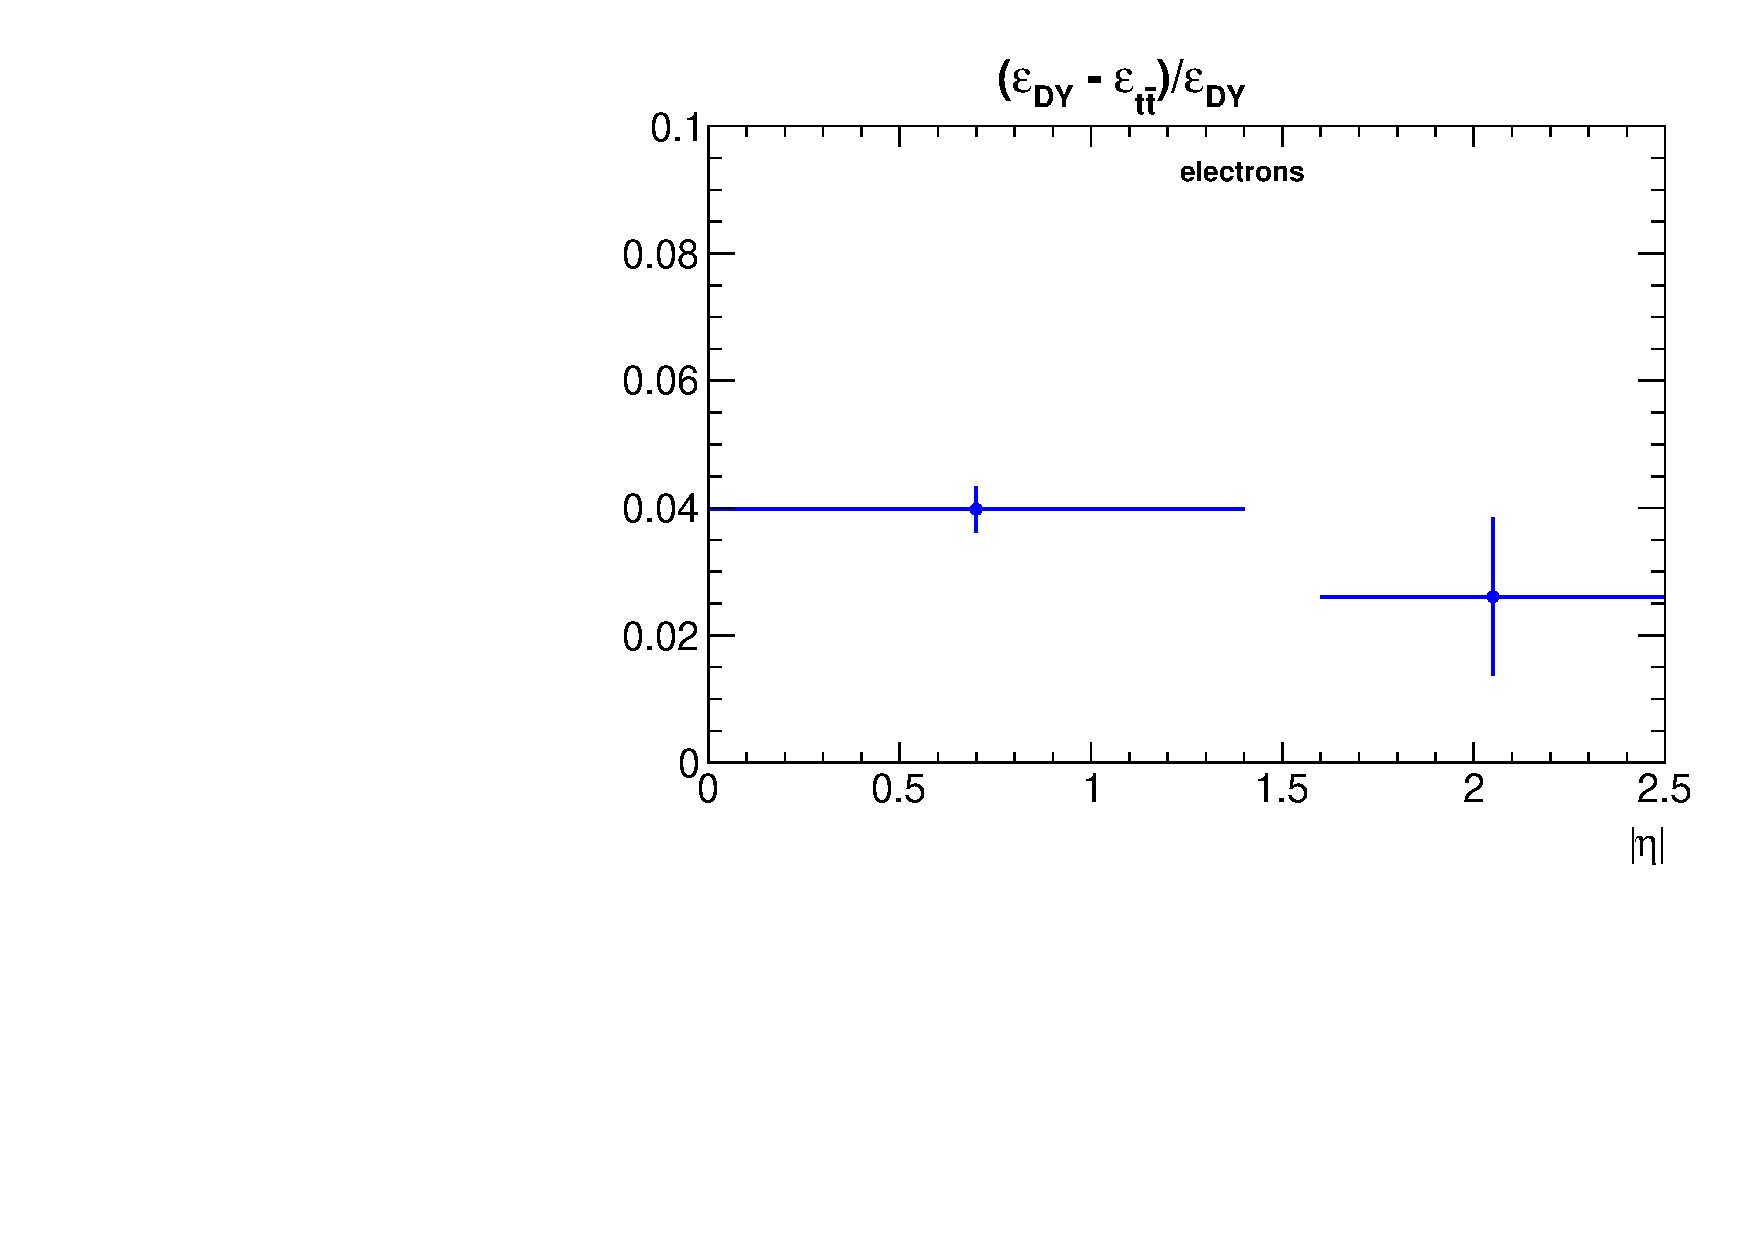
\includegraphics[width=0.49\linewidth]{p_eff_el_rel_diff_vs_eta}
\caption[The electron efficiency measured vs \pt~and \aeta]
{\label{fig:eff_comp_el}
The electron efficiency measured using DY (red) and \ttbar~MC (black). The
top two plots are the efficiencies projected vs \pt~and \aeta, respectively.
The bottom two plots are the relative differences between DY and \ttbar~ also
projected vs \pt~and \aeta.}
\end{center}
\end{figure}
% --------------------------------------------------------------------------- %
\begin{table}[!hbt]
\caption[The muon efficiency relative differences between DY and \ttbar]
{\label{tab:eff_comp_mu}
The muon efficiency relative differences between DY and \ttbar~
($(\epsilon_{DY} - \epsilon_{\ttbar})/\epsilon_{DY}$). The uncertainties are
statistical only.
}
\begin{center}
\begin{tabular}{c|c|c}
\hline\hline
\backslashbox{\pt}{\aeta} & 0.00 - 1.20       & 1.20 - 2.50       \\\hline
10 - 20 \GeV              & 0.113 $\pm$ 0.014 & 0.104 $\pm$ 0.016 \\
20 - 30 \GeV              & 0.109 $\pm$ 0.009 & 0.078 $\pm$ 0.012 \\
30 - 40 \GeV              & 0.084 $\pm$ 0.007 & 0.067 $\pm$ 0.011 \\
40 - 50 \GeV              & 0.075 $\pm$ 0.007 & 0.058 $\pm$ 0.011 \\
50 - 70 \GeV              & 0.047 $\pm$ 0.006 & 0.026 $\pm$ 0.009 \\
70 - 100 \GeV             & 0.036 $\pm$ 0.009 & 0.012 $\pm$ 0.013 \\
100- 200 \GeV             & 0.026 $\pm$ 0.014 & 0.042 $\pm$ 0.020 \\ \hline\hline
\end{tabular}
\end{center}
\end{table}
% --------------------------------------------------------------------------- %
\begin{figure}[!hbt]
\begin{center}
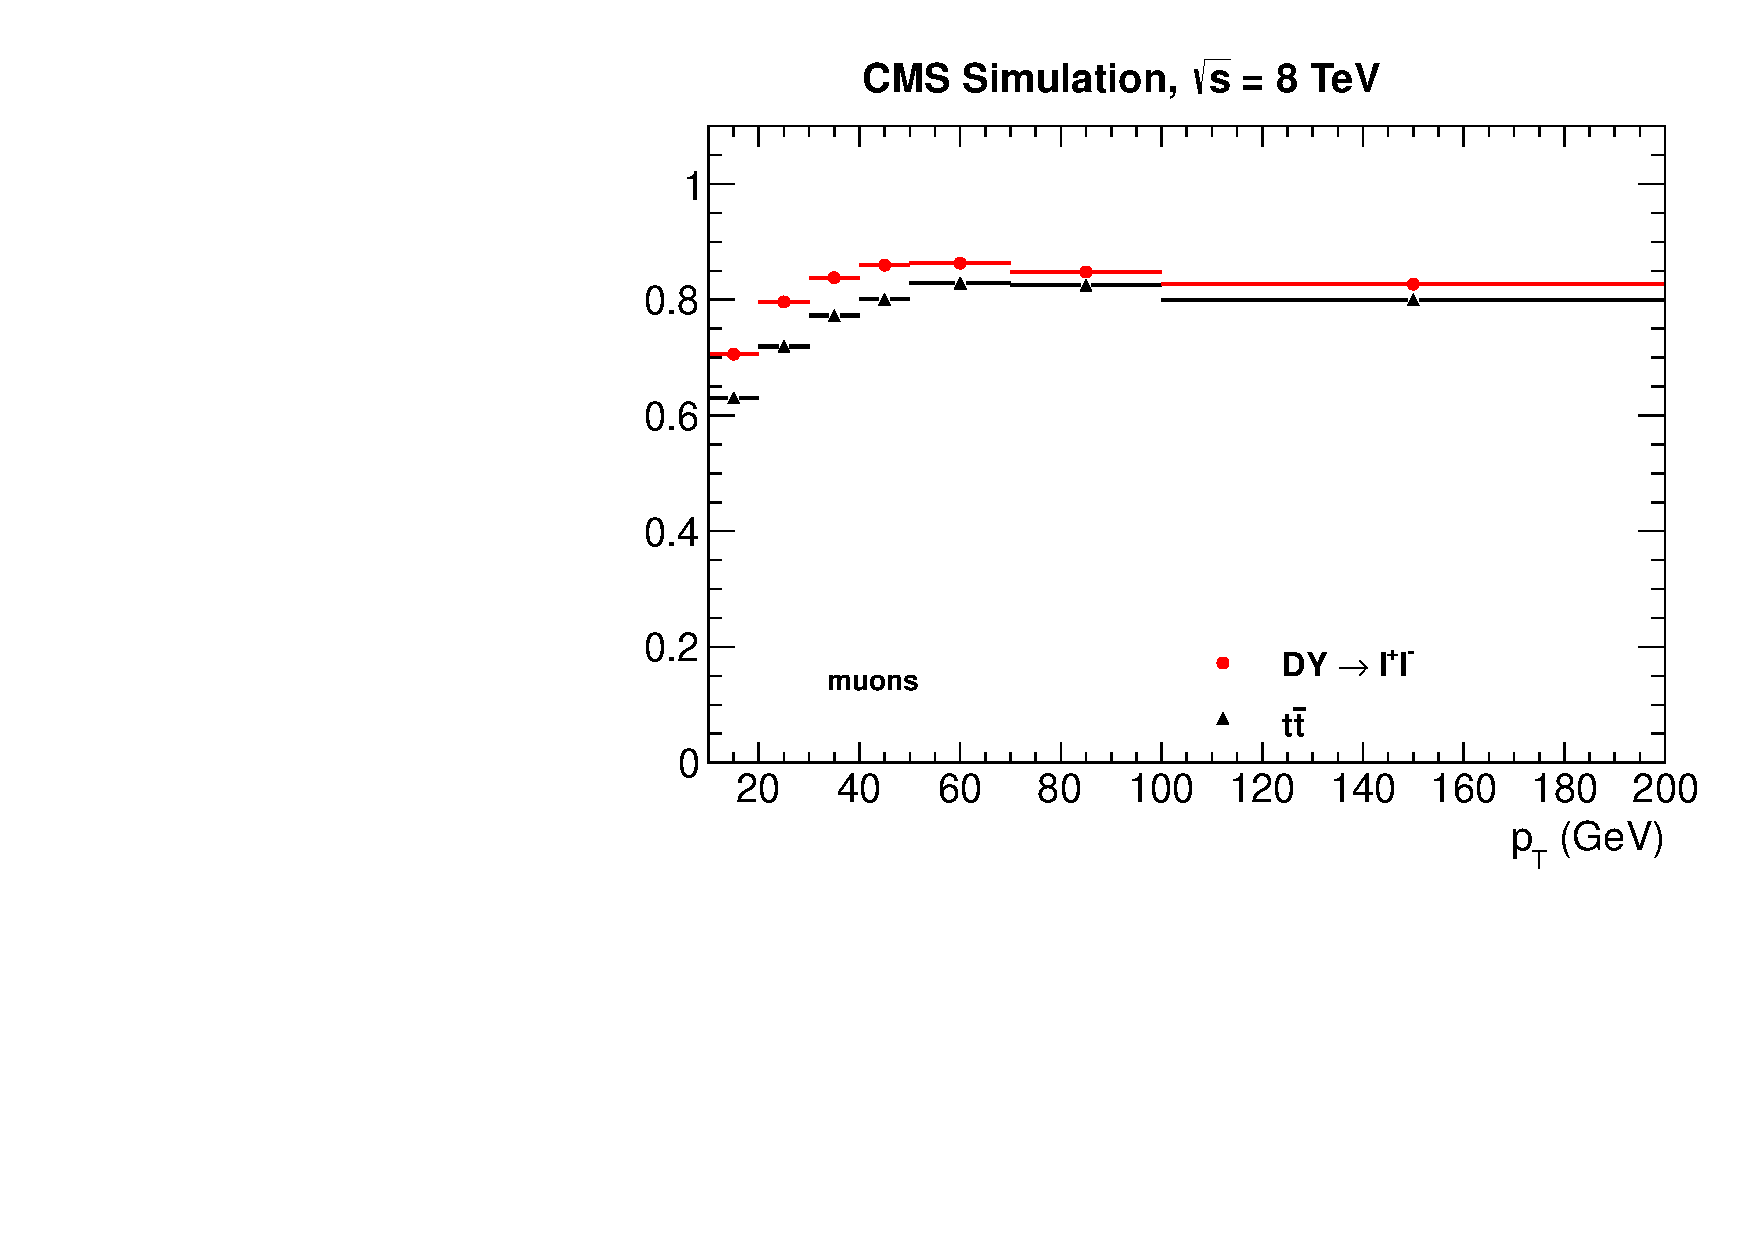
\includegraphics[width=0.49\linewidth]{p_eff_mu_vs_pt}
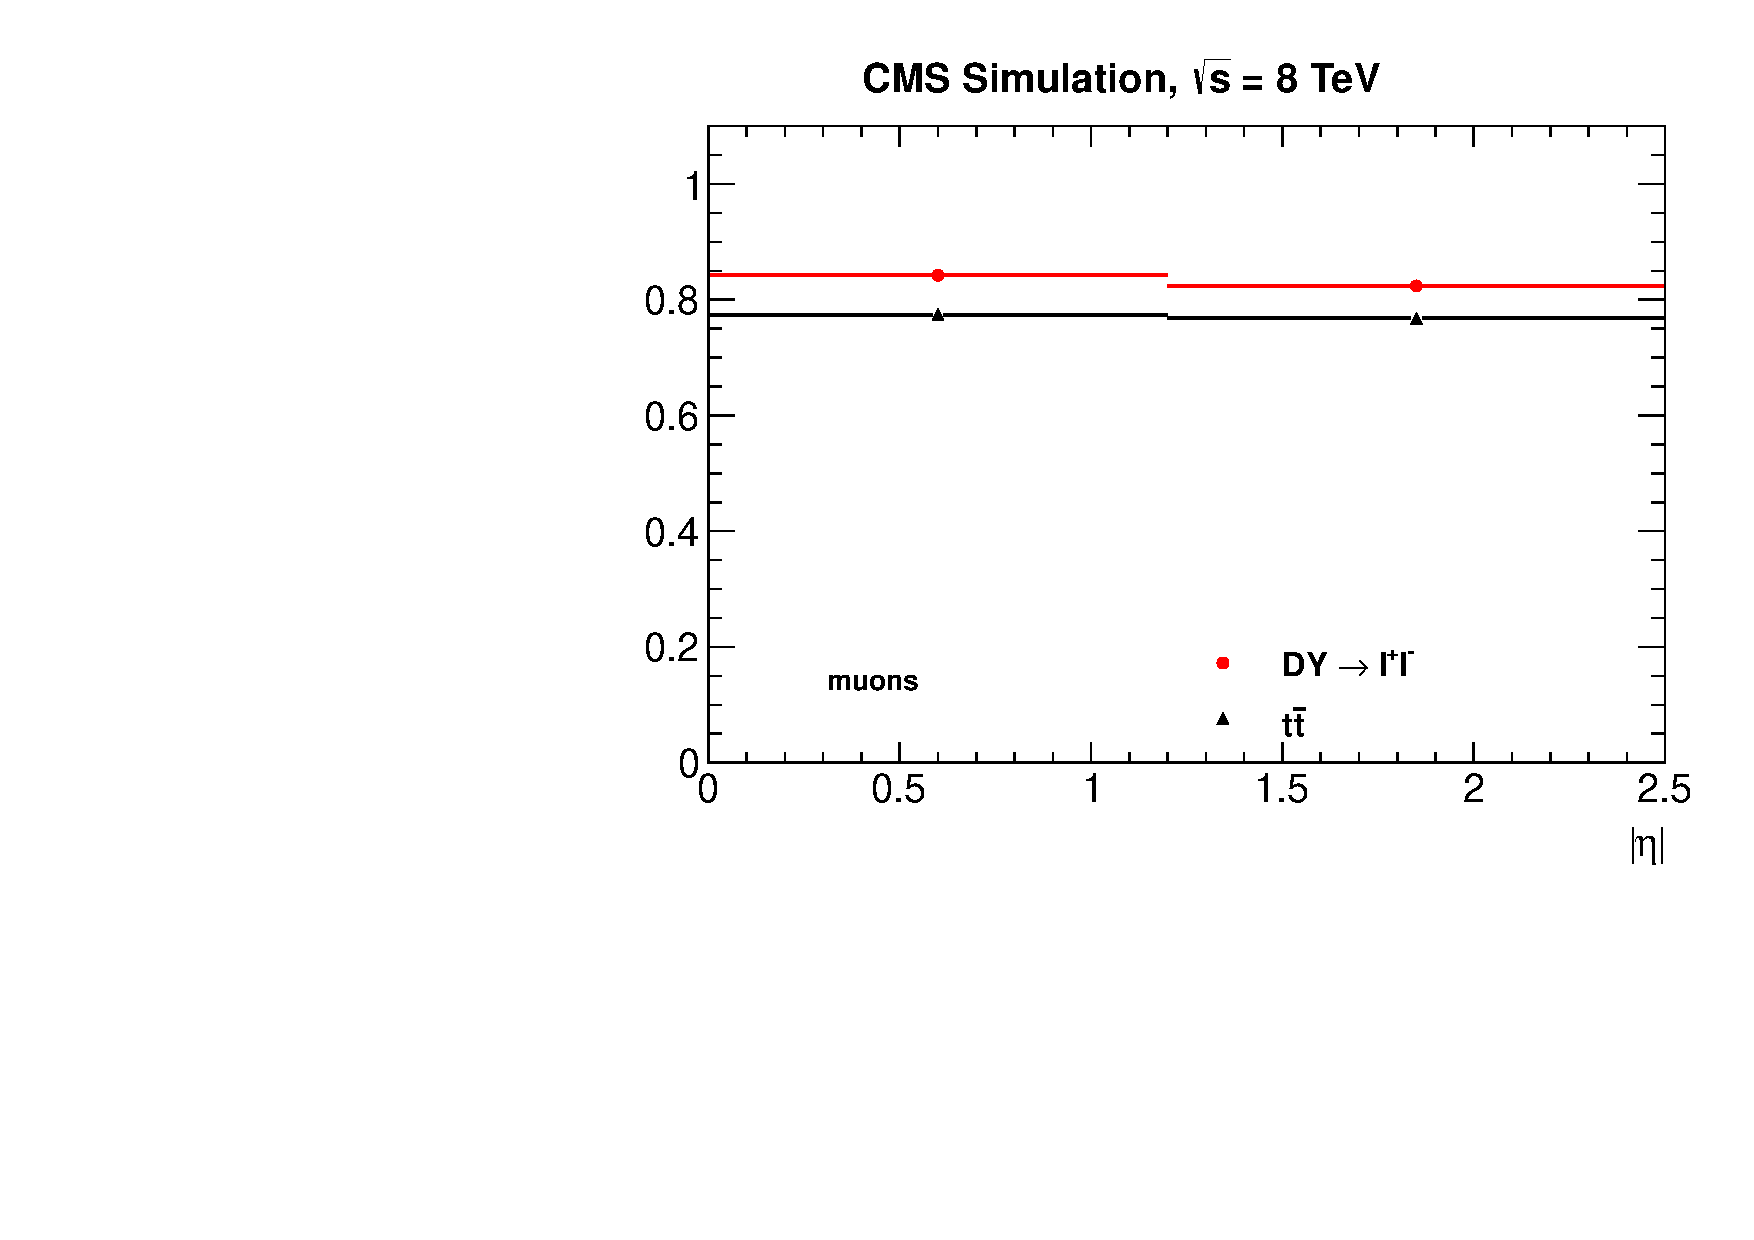
\includegraphics[width=0.49\linewidth]{p_eff_mu_vs_eta}
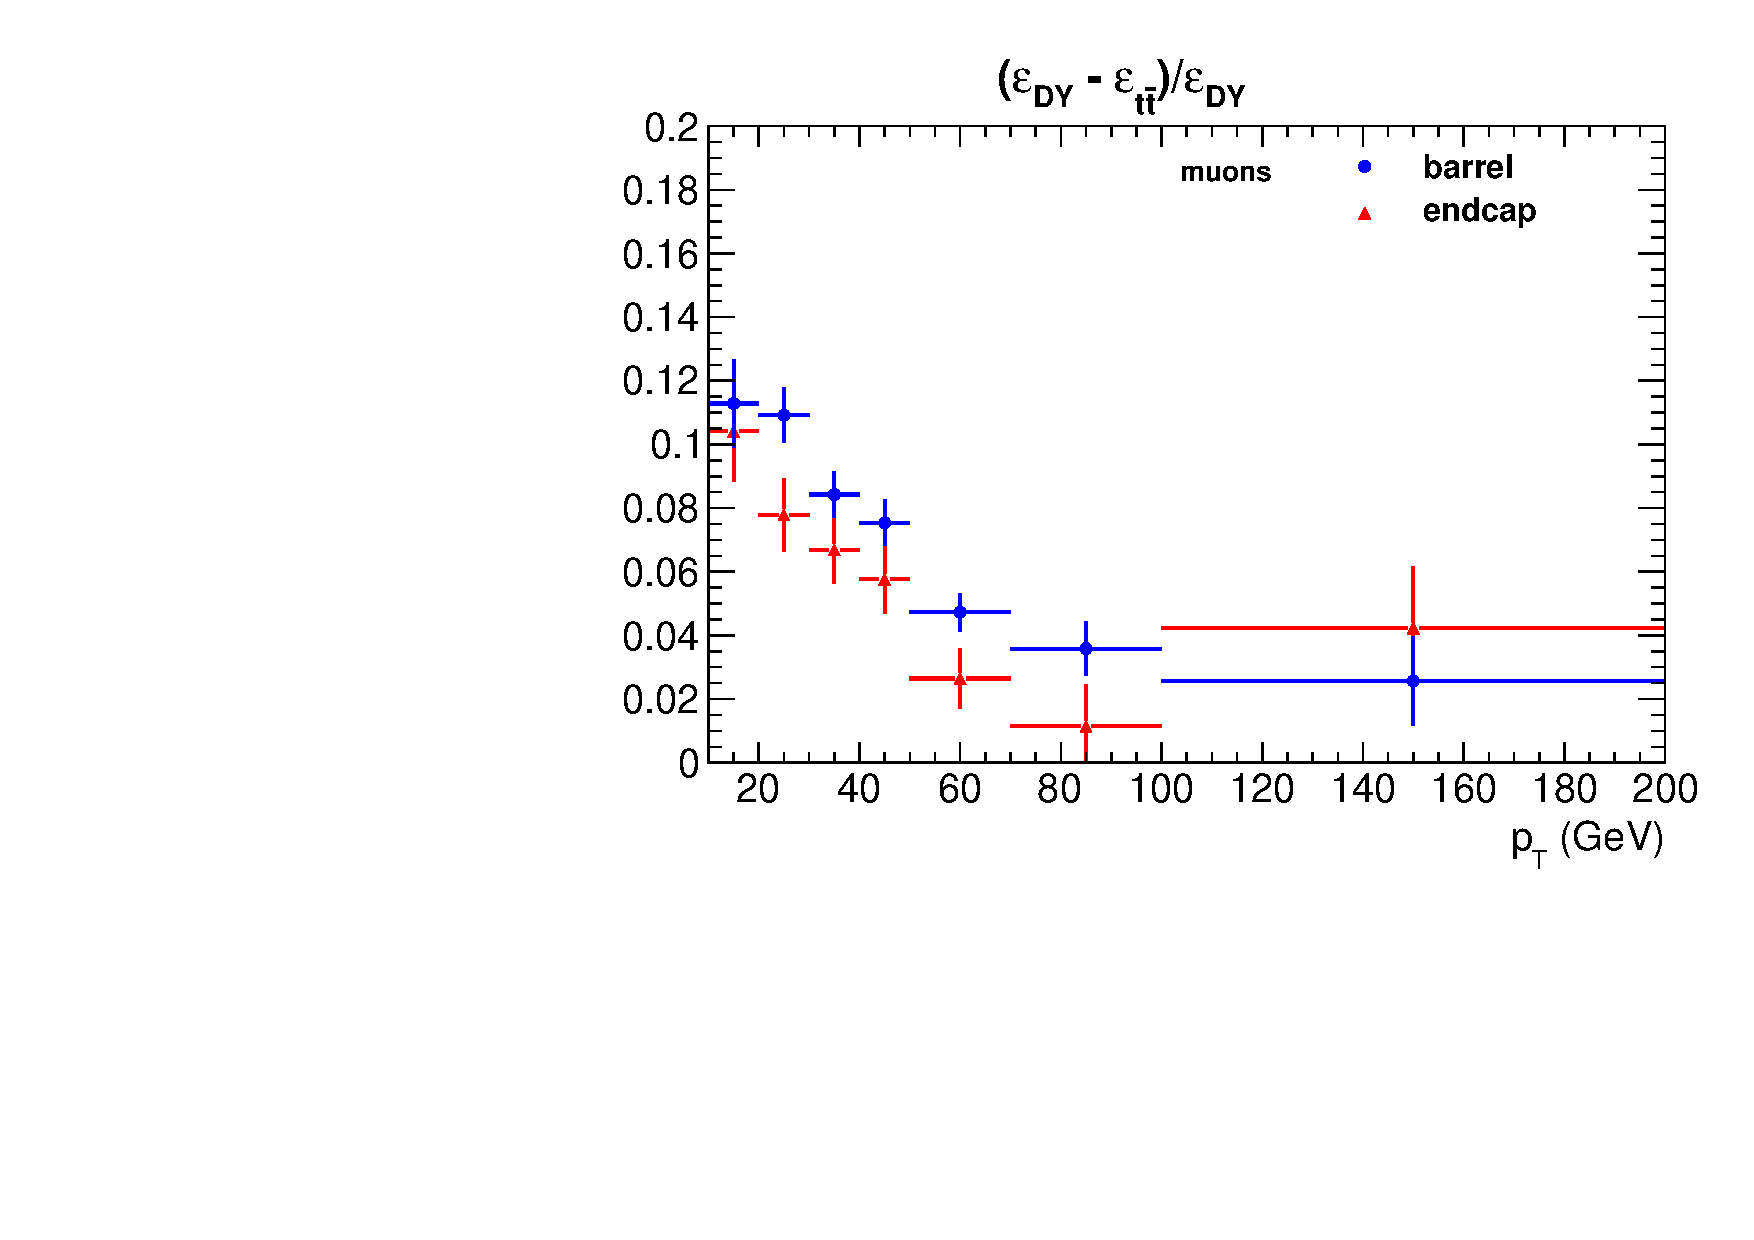
\includegraphics[width=0.49\linewidth]{p_eff_mu_rel_diff_vs_pt_compare}
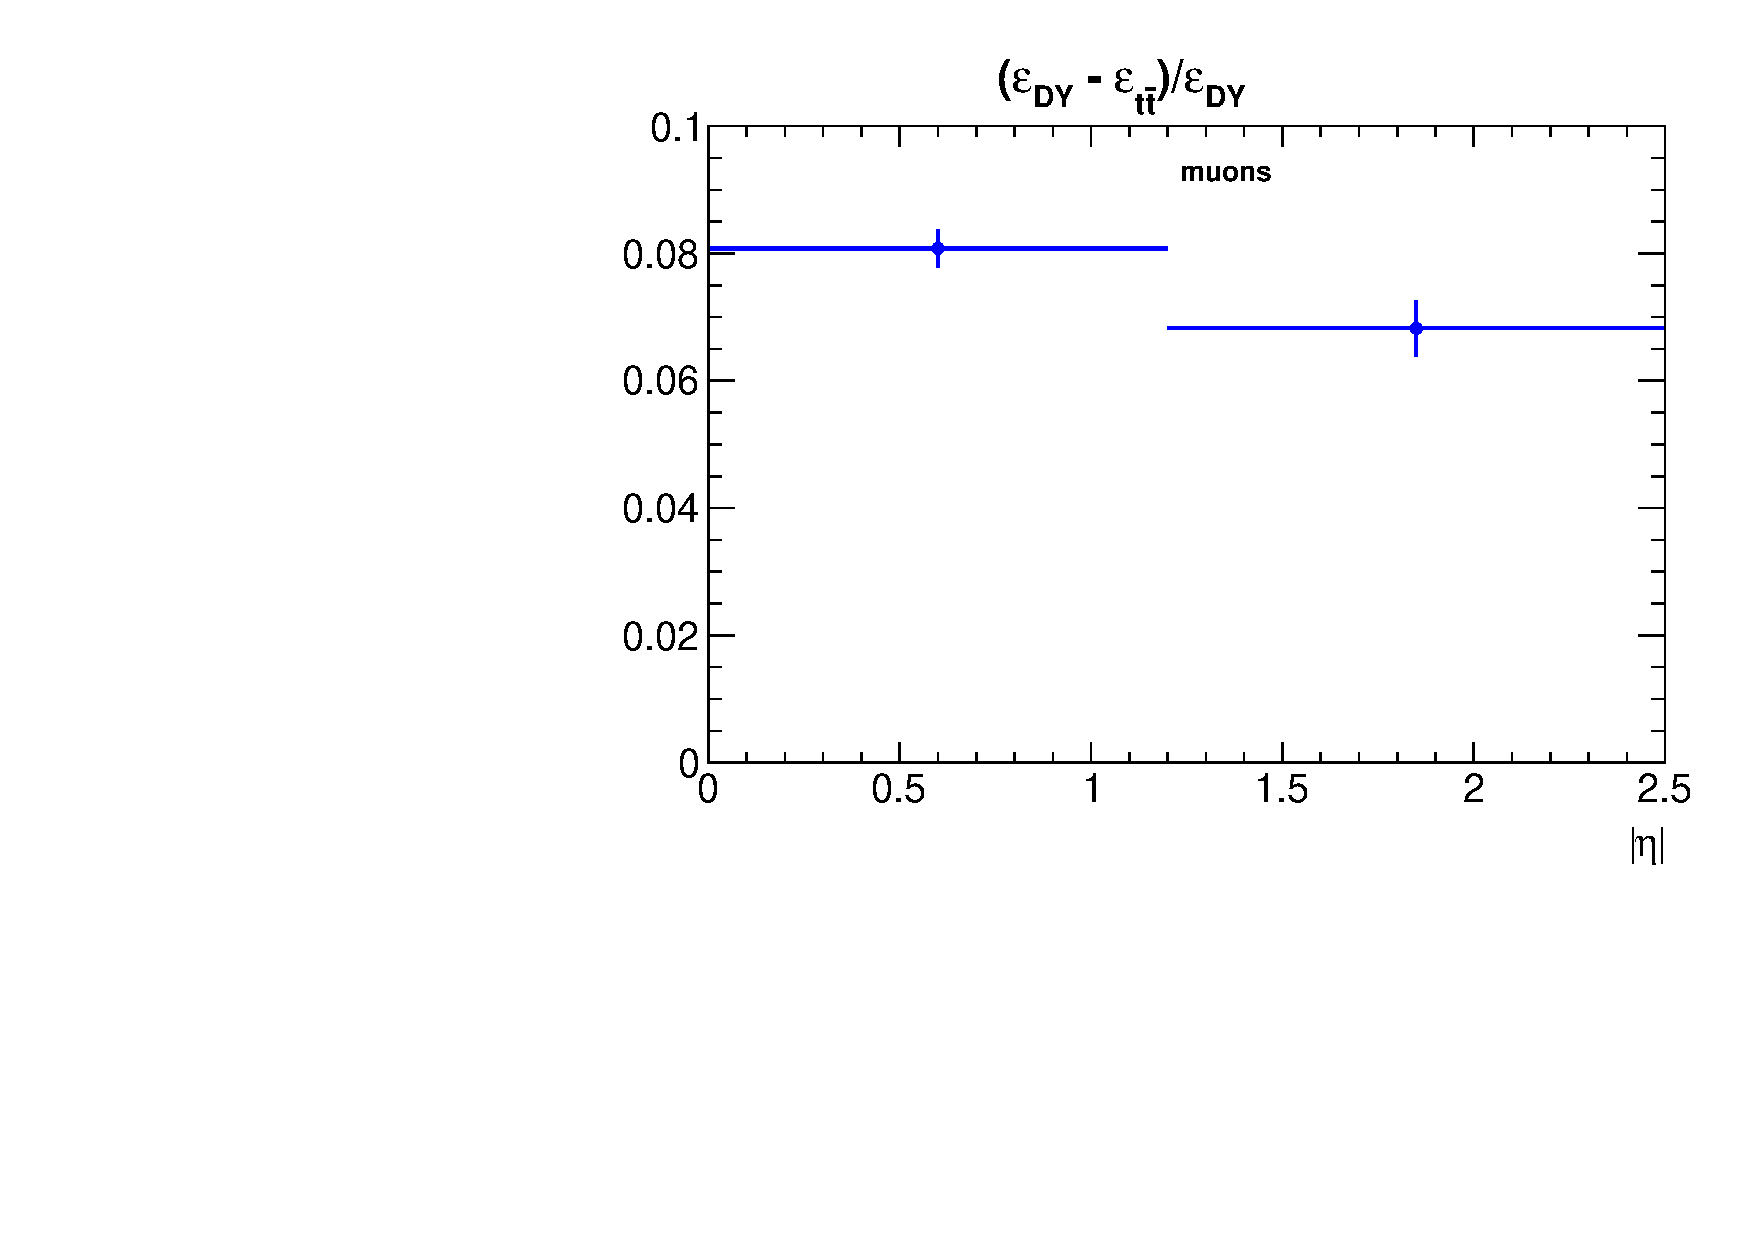
\includegraphics[width=0.49\linewidth]{p_eff_mu_rel_diff_vs_eta}
\caption[The muon efficiency measured vs \pt~and \aeta]
{\label{fig:eff_comp_mu}
The muon efficiency measured using DY (red) and \ttbar~MC (black). The top two
plots are the efficiencies projected vs \pt~and \aeta, respectively. The bottom
two plots are the relative differences between DY and \ttbar~ also projected vs
\pt~and \aeta.
}
\end{center}
\end{figure}
 
% --------------------------------------------------------------------------- %
Here we see that the majority of the differences come at low \pt~where we
see relative differences on the order of 10\% for muons and 5\% for the
electrons. As we move to higher \pt~the differences are only on the order
of a few percent. To account for these differences we assign a systematic
uncertainty which is roughly half the relative difference stated in
tables~\ref{tab:eff_comp_el},~\ref{tab:eff_comp_mu}:
% --------------------------------------------------------------------------- %
\begin{itemize}
  \item muons: 5\% for $\pt < 30\ $\GeV~ and 3\% for $\pt > 30\ \GeV$
  \item electrons: 3\%
\end{itemize}

% --------------------------------------------------------------------------- %
To account for the differences in the efficiency between data and
simulation, the scale factors reported in Tables~\ref{tab:eff_comp_el}
and~\ref{tab:eff_comp_mu} are applied to each MC sample used in the prediction
with Table~\ref{tab:eff_lepsyst} summarizing the various systematic
uncertainties taken.
% --------------------------------------------------------------------------- %
\begin{table}[ht!]
\caption[The systematic uncertainties applied to the data-to-MC efficiency scale factors]
{\label{tab:eff_lepsyst}
The systematic uncertainties applied to the data-to-MC efficiency scale factors.
}
\begin{center}
\begin{tabular}{c|c|c|c}
\hline\hline
\multirow{3}{*}{\tnp}        & lepton flavor & $p_T < 15\ GeV$ & $p_T > 15\ GeV$ \\ \hline
                             & electron      & $10\%$          & $5\%$           \\
                             & muon          & $5\%$           & $3\%$           \\ \hline \hline
\multirow{3}{*}{composition} &               & $p_T < 30\ GeV$ & $p_T > 30\ GeV$ \\ \hline
                             & electron      & $3\%$           & $3\%$           \\
                             & muon          & $5\%$           & $3\%$           \\ \hline\hline
\end{tabular}
\end{center}
\end{table}
% --------------------------------------------------------------------------- %

% --------------------------------------------------------------------------- %
% --------------------------------------------------------------------------- %
\section{Trigger Efficiencies}
\label {sec:eff_trig}
% --------------------------------------------------------------------------- %
% --------------------------------------------------------------------------- %
The trigger efficiencies and data-to-MC scale factor is calculated for
every trigger and is applied \pt and \aeta dependent for each lepton.
Details on how the scale factors have been studied and calculated can be
found in~\cite{an_ufl2013}. The value of those scale factors is shown in
Table~\ref{tab:eff_trig}.
% --------------------------------------------------------------------------- %
\begin{table}[!hbt]
\begin{center}
\caption[Scale factors from trigger inefficiencies applied to Monte Carlo predictions from the rare backgrounds]
{\label{tab:eff_trig}
Scale factors from trigger inefficiencies applied to Monte Carlo predictions
from the \emph{irreducible} backgrounds. For some channels, scale factors are
parametrized by the trailing lepton \pt or \aeta.
}
\begin{tabular}{|l|c|l|c|} \hline\hline
Low-$\pt$            & Scale Factor & High-$\pt$           & Scale Factor  \\ \hline \hline
$\mu\mu$, $|\eta|<1$ & 0.94         & $\mu\mu$, $|\eta|<1$ & 0.90          \\ \hline
$\mu\mu$, $|\eta|>1$ & 0.90         & $\mu\mu$, $|\eta|>1$ & 0.81          \\ \hline
$e\mu$               & 0.93         & $e\mu$               & 0.93          \\ \hline
$ee$                 & 0.93         & $ee$, $\pt<30$       & 0.92          \\ \hline
                     &              & $ee$, $\pt>30$       & 0.96          \\ \hline\hline
\end{tabular}
\end{center}
\end{table}

% --------------------------------------------------------------------------- %
% --------------------------------------------------------------------------- %
\section{B-tagging Efficiency}
\label {sec:eff_btag}
% --------------------------------------------------------------------------- %
% --------------------------------------------------------------------------- %
Since the b-tagging efficiencies measured in data are somewhat different than
those measured by simulation, a scale factor is applied to simulated events to
take this difference into account. The CMS B-tagging and Vertex Group (BTV) has
measured the b-tagging scale factors between data and MC. The scale factors in
general depend on the jet flavor, \pt, and \aeta and the details are described
by the BTV in~\cite{beff_2012,btvtwiki}. These scale factors were measured on
muon-jet and \ttbar~ data and are documented in~\cite{btvtwiki}. In contrast to
the previous iterations of this analysis where the scale factor was applied as
an additional event weight, the scale factor will now be used to update the
b-tagging status on a jet-by-jet basis. A full description is provided in the
stated reference; however, we provide a short summary of the method here. In
this method, scale factors are used to update the b-tagging status on each jet
individually. In order to upgrade or downgrade the b-tagging status of each
individual jet, a random number generator is used. This gives the advantage
that the yields from MC can be treated the same way as data. The method in our
case is relatively simple since we only have one operating point. If $SF < 1$,
then the fraction of $f = 1 - SF$ b-tagged jets from the ``tagged'' collection
are to be downgraded to the ``non-tagged'' status and in this case, it is
not necessary to know the MC b-tagging efficiency. The situation gets more
complicated when $SF > 1$. It is necessary to upgrade the b-tagging status of
some of the untagged jets and the fraction of such jets that needs to be upgraded
is
% --------------------------------------------------------------------------- %
\[
  f = \frac{1 - SF}{1 - 1/\varepsilon_{MC}}.
\]
% --------------------------------------------------------------------------- %
Using this relationship and a random number, we recount the number of b-tagged
jets on all events and use the count of this new collection in all selections
regarding the \nbtags. To estimate the systematic uncertainty on the b-tagging
efficiency scale factor, the uncertainty is scaled up or down and then
the above procedure is repeated. The difference between the unscaled and
the scaled acceptance efficiency is used in determining the systematic
uncertainty. These are considered fully correlated between the search regions.
Figure~\ref{fig:eff_nbtags} shows the effect of the this rescaling procedure on the
\nbtags distribution on a \ttW MC sample which is required to pass the baseline
selections (SR0).
% --------------------------------------------------------------------------- %
\begin{figure}[!htb]
\begin{center}
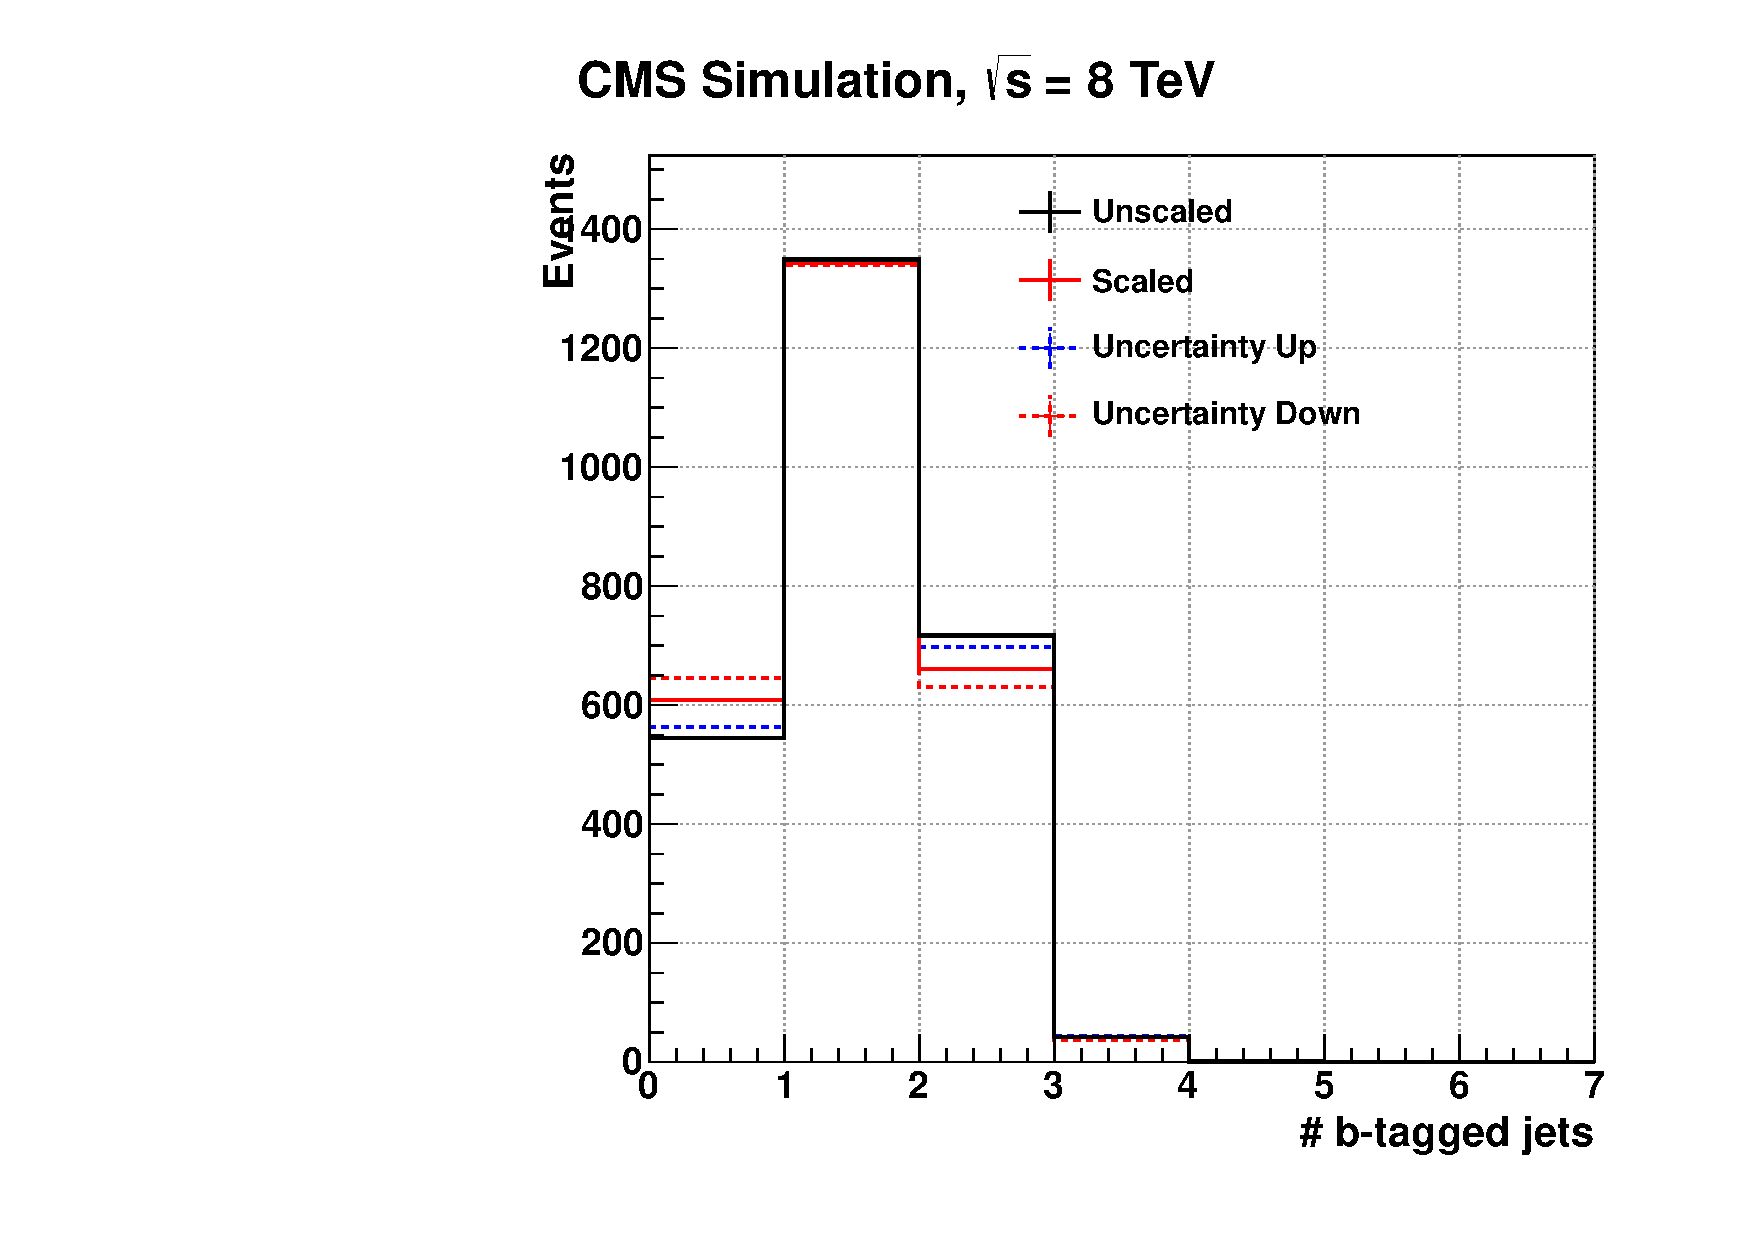
\includegraphics[width=0.8\linewidth]{p_nbtags.pdf}
\end{center}
\caption[\nbtags~distribution for \ttW~MC sample to illustrate the effect of the b-tag rescaling procedure]
{\label{fig:eff_nbtags}
\nbtags~distribution for \ttW~MC sample to illustrate the effect of the b-tag
rescaling procedure on the number of b-tagged jets.
}
\end{figure}
% --------------------------------------------------------------------------- %
